\documentclass[a4paper, 12pt, titlepage]{article}

% Including needed packages
\usepackage[margin=2cm]{geometry}
\usepackage{amsmath}
\usepackage{amssymb}
\usepackage{amsthm}
\usepackage{graphicx}
\usepackage{subfig}
\usepackage{float}


\DeclareMathOperator{\spanop}{span}

\title
{{\em Machine learning 2}\\
Exercise sheet 4}
\author{FLEISCHMANN Kay, Matrnr: 352247\\
	ROHRMANN Till, Matrnr: 343756}
\date{\today}

\begin{document}

\maketitle

\setcounter{section}{5}


\section{Kernel Canonical Correlation Analysis}

\subsection*{(6a.) Derive the dual optimization problem}
Given some training data $X \in \mathbb{R}^{d1 \times N} $ and $Y \in \mathbb{R}^{d2 \times N}$. 
The idea behind CCA is to find two features $w_x$ and $w_y$ in input space such that their correlation is maximised.
Let $C_{xx} = XX^T$, $C_{yy} = YY^T$, $C_{xy} = XY^T$ and $C_{yx} = YX^T$.
\newline \newline
Formally: Find $w_x \in \mathbb{R}^{d_1}$, $w_y \in \mathbb{R}^{d_2}$ which maximize
\begin{eqnarray}
  w^{T}_{x} C_{xy}w_y \label{eq:prob}
 \end{eqnarray}
with subject to
\begin{eqnarray}
  w^T_xC_{xx}w_x=1 \label{eq:constraint1}\\
  w^T_yC_{yy}w_y=1 \label{eq:constraint2}
\end{eqnarray}
Show that it is always possible to find an optimal solution in the span of the data, that is $w_x= X \alpha_x$, $w_y = Y \alpha_y$:
\begin{proof}[Proof by contradiction]
Let's assume

\begin{eqnarray}
	\max_{\alpha_x, \alpha_y \in \mathbb{R}^{N}} \alpha_x^TX^TC_{xy}Y\alpha_y &<&
	\max_{v \in \mathbb{R}^{d_1}, w\in \mathbb{R}^{d_2}} v^T C_{xy} w \label{eq:0}
\end{eqnarray}

We can seperate the space $\mathbb{R}^{d_1} = \spanop{\{X\}} \cup \spanop{\{X\}}^\bot$ into the span of the column vectors of $X$ and its orthogonal space.
The same holds for $\mathbb{R}^{d_2} = \spanop{\{Y\}} \cup \spanop{\{Y\}}^\bot$.
Thus every $v\in \mathbb{R}^{d_1}$ can be represented by its projection $v_{X}$ into $\spanop{\{X\}}$ and its projection $v_{X^\bot}$ in $\spanop{\{X\}}^\bot$.

\begin{eqnarray*}
	v &=& v_{X} + v_{X^\bot}
\end{eqnarray*}

We can now deduce the following:

\begin{eqnarray}
	\max_{v \in \mathbb{R}^{d_1}, w\in \mathbb{R}^{d_2}} v^T C_{xy} w &=&
	\max_{v \in \mathbb{R}^{d_1}, w\in \mathbb{R}^{d_2}} \left(v_{X} + v_{X^\bot} \right)^T XY^T\left(w_{Y} + w_{Y^\bot} \right) \label{eq:1}
\end{eqnarray}

Because $v_{X^\bot}$ belongs to the orthogonal space $\spanop{\{X\}}^\bot$, the term $X^Tv_{X^\bot}=0$.
The same holds for $w_{Y^\bot}$, that is to say $Y^Tw_{Y^\bot}=0$.
This leads to:

\begin{eqnarray}
	\eqref{eq:1} &=& \max_{v_X \in \spanop{\{X\}}, w_Y \in \spanop{\{Y\}}} v_X^TXY^Tw_Y \nonumber\\
	&=& \max_{\alpha_x,\alpha_y \in \mathbb{R}^N} \alpha_x^TX^TC_{xy}Y\alpha_y \label{eq:2}
\end{eqnarray}
Where the equation \eqref{eq:2} is just another form to express that $v_X$ lies in the space $\spanop{\{X\}}$ and $w_Y$ lies in the space $\spanop{\{Y\}}$.
By equating equation \eqref{eq:0} with \eqref{eq:2} we get
\begin{eqnarray*}
	\max_{\alpha_x, \alpha_y \in \mathbb{R}^{N}} \alpha_x^TX^TC_{xy}Y\alpha_y &<&
	\max_{\alpha_x,\alpha_y \in \mathbb{R}^N} \alpha_x^TX^TC_{xy}Y\alpha_y
\end{eqnarray*}
Which is obviously a contradiction.
Thus we can always find an optimal solution for the equation \eqref{eq:prob} in the span of the data $X$ and $Y$ respectively.
\end{proof}
Derive the dual optimization problem: \newline
\begin{eqnarray*}
  \mathcal{L}(\alpha, \beta) &=& w^{T}_{x} C_{xy}w_y - \frac{1}{2} \alpha (w^T_xC_{xx}w_x-1) -\frac{1}{2} \beta (w^T_yC_{yy}w_y-1)
  \end{eqnarray*}
\begin{eqnarray}
  \frac{\partial L}{\partial w^T_x} = XY^Tw_y - \alpha( XX^Tw_x ) = 0  \Leftrightarrow XY^Tw_y = \alpha( XX^Tw_x ) \label{eq:3} \\
  \frac{\partial L}{\partial w^T_y} = YX^Tw_x - \beta ( YY^Tw_y) = 0 \Leftrightarrow  YX^Tw_x = \beta ( YY^Tw_y) \label{eq:4}
\end{eqnarray}
Multiplication $w^T_x$ with equation \eqref{eq:3} and $w^T_y$ with Equation \eqref{eq:4} results to:
\begin{eqnarray*}
  w^T_xXY^Tw_y = \alpha( w^T_xXX^Tw_x ) \\
  w^T_yYX^Tw_x = \beta ( w^T_yYY^Tw_y) 
\end{eqnarray*}
Because of constraints \eqref{eq:constraint1} and \eqref{eq:constraint2} 
\begin{eqnarray}
  \alpha( w_x^TXX^Tw_x )=\beta ( w^T_yYY^Tw_y)  \Rightarrow \alpha = \beta \label{eq:eq}
\end{eqnarray}
Next we combine equations \eqref{eq:3}, \eqref{eq:4} and \eqref{eq:eq}.
\begin{eqnarray*}
  C_{xy}w_y = \alpha C_{xx}  w_x \\
  C_{yx}w_x = \alpha C_{yy}  w_y
\end{eqnarray*}
Written in matrix form, we finally get a generalized eigenvalue problem: \newline \newline
\begin{eqnarray}
\begin{bmatrix} 0 & C_{xy} \\ C_{yx} & 0 \end{bmatrix}
\begin{bmatrix} w_x \\ w_y \end{bmatrix} 
&=&  \alpha
\begin{bmatrix} C_{xx} & 0 \\ 0 & C_{yy} \end{bmatrix}
\begin{bmatrix} w_x \\ w_y \end{bmatrix} \label{eq:maeq}
\end{eqnarray}

\subsection*{Show that the dual optimization
problem is equivalent to finding the solution of the generalized eigenvalue problem}
Since we know that there exists an optimal solution in the data span, we can represent our $w_x$ and $w_y$ by:
\begin{eqnarray}
	w_x &=& X\alpha_x \label{eq:s1}\\
	w_y &=& Y\alpha_y \label{eq:s2}
\end{eqnarray}

for some $\alpha_x, \alpha_y \in \mathbb{R}^{N}$.
By substituting equations \eqref{eq:s1} and \eqref{eq:s2} into equation \eqref{eq:maeq} with a subsequent left multiplication of the matrix 
\begin{eqnarray*}
	\begin{bmatrix}
		X^T & 0\\
		0 & Y^T
	\end{bmatrix}
\end{eqnarray*}
we obtain the following:
\begin{eqnarray*}
	\begin{bmatrix}
		0 & X^TXY^T\\
		Y^TYX^T & 0
	\end{bmatrix}
	\begin{bmatrix}
		X\alpha_x\\
		Y\alpha_y
	\end{bmatrix} &=& \rho
	\begin{bmatrix}
		X^T X X^T & 0\\
		0 & Y^T Y Y^T
	\end{bmatrix}
	\begin{bmatrix}
		X\alpha_x\\
		Y\alpha_y
	\end{bmatrix}
\end{eqnarray*}
Which is equivalent to
\begin{eqnarray*}
	\begin{bmatrix}
		0 & X^TXY^TY\\
		Y^TYX^TX & 0
	\end{bmatrix}
	\begin{bmatrix}
		\alpha_x\\
		\alpha_y
	\end{bmatrix} &=& \rho
	\begin{bmatrix}
		X^T X X^T X & 0\\
		0 & Y^T Y Y^T Y
	\end{bmatrix}
	\begin{bmatrix}
		\alpha_x\\
		\alpha_y
	\end{bmatrix}
\end{eqnarray*}

With $K_X = X^TX$ and $K_Y = Y^TY$ we finally obtain
\begin{eqnarray*}
	\begin{bmatrix}
		0 & K_XK_Y\\
		K_YK_X & 0
	\end{bmatrix}
	\begin{bmatrix}
		\alpha_x\\
		\alpha_y
	\end{bmatrix} &=& \rho
	\begin{bmatrix}
		K_X^2 & 0\\
		0 &K_Y^2
	\end{bmatrix}
	\begin{bmatrix}
		\alpha_x\\
		\alpha_y
	\end{bmatrix}
\end{eqnarray*}

\subsection*{(6b.) Describe how the generalized eigenvalue problem from exercise (a) - and thus CCA - can be kernelized.}
The kernel trick extends a machine learning algorithm by introducing a mapping of the data points into a higher dimensional feature-space, without knowing the mapping-functions explicitely.  This happens with the idea of just knowing a scalar product in this space and we are able to change the formulation of the machine learning algorithm which now just needs the scalar-products between the datapoints.


To apply the CCA to a feature space without explicitely calculating the mapping between input and feature space, we can easily adapt the existing method.
Given that we have a kernel function $k(\cdot,\cdot)$ representing the inner product in our feature space, we only have to substitute $K_X$ by $(\tilde{K}_X)_{i,j} = k(x_i,x_j)$ and $K_Y$ by $(\tilde{K}_Y)_{i,j} = k(y_i,y_j)$ where $x_i$ is the $i$-th column of $X$ and $y_i$ the $i$-th column of $Y$.
This can easily be done because the original problem has been transformed into the dual problem which uses only scalar products.
The resulting generalized eigenvalue problem is then:

\begin{eqnarray*}
	\begin{bmatrix}
		0 & \tilde{K}_X\tilde{K}_Y\\
		\tilde{K}_Y\tilde{K}_X & 0
	\end{bmatrix}
	\begin{bmatrix}
		\alpha_x\\
		\alpha_y
	\end{bmatrix} &=& \rho
	\begin{bmatrix}
		\tilde{K}_X^2 & 0\\
		0 &\tilde{K}_Y^2
	\end{bmatrix}
	\begin{bmatrix}
		\alpha_x\\
		\alpha_y
	\end{bmatrix}
\end{eqnarray*}

\section{tkCCA}

\begin{figure}
	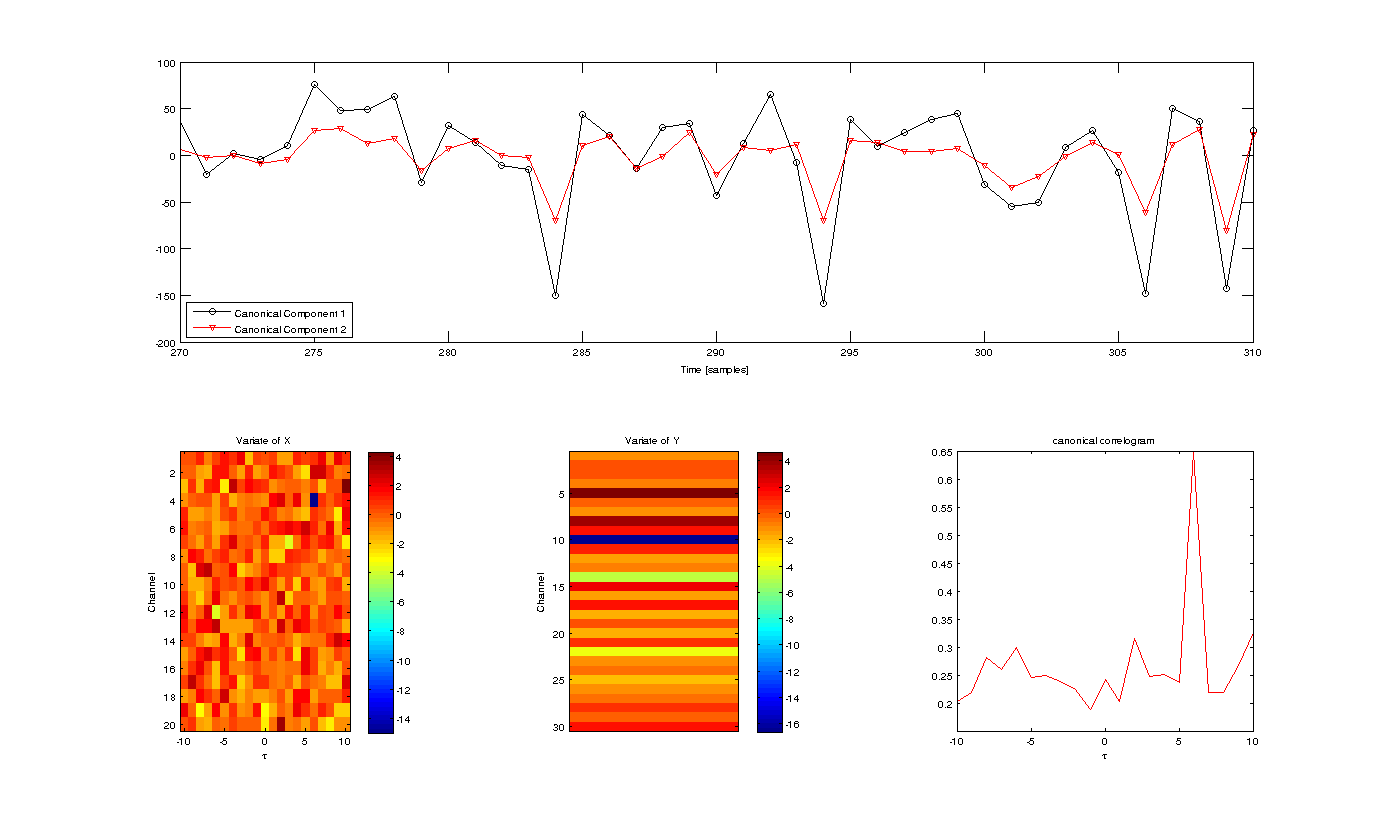
\includegraphics[width=17cm]{images/tkcca.png}
	\caption{Results of the tkCCA.}
\end{figure}

We can clearly see in the canonical correlogram that there exists a strong correlation between $X$ and $Y$ at the time shift $\tau=6$.
Since there exists no other maximum which has a comparable magnitude, we can conclude that the hidden one-dimensional signal occurs probably with a delay of $6$ time units in the data set $Y$.

\end{document}
